\documentclass[article,nojss]{jss}
\DeclareGraphicsExtensions{.pdf,.eps}
\newcommand{\mysection}[1]{\subsubsection[#1]{\textbf{#1}}}


%% need no \usepackage{Sweave}

\author{Gabor Grothendieck\\GKX Associates Inc. \And
        Achim Zeileis\\Wirtschaftsuniversit\"at Wien}
\Plainauthor{Achim Zeileis, Gabor Grothendieck}

\title{\pkg{zoo} FAQ}
\Plaintitle{zoo FAQ}

\Keywords{irregular time series, daily data, weekly data, returns}

\Abstract{This is a collection of frequently asked questions (FAQ) about the \pkg{zoo} package together with their answers. }

\Address{
  Gabor Grothendieck\\
  GKX Associates Inc.\\
  E-mail: \email{ggrothendieck@gmail.com}\\
  
  Achim Zeileis\\
  Wirtschaftsuniversit\"at Wien\\
  E-mail: \email{Achim.Zeileis@R-project.org}\\  
}
  
\begin{document}


%\VignetteIndexEntry{zoo FAQ}
%\VignetteDepends{zoo,tseries}
%\VignetteKeywords{irregular time series, daily data, weekly data, returns}
%\VignettePackage{zoo}



\mysection{1. I know that duplicate times are not allowed but my data has them.  What do I do?}

\pkg{zoo} objects should not normally contain duplicate times.
If you try to create such an object using
\pkg{zoo} or \code{read.zoo} then warnings will be issued but
the objects will be created.   The user then has the opportunity
to fix them up -- typically by using \code{aggregate.zoo}
or \code{duplicated}.  

Merging is not well defined for duplicate series with duplicate
times and rather than give an undesired or unexpected result,
\code{merge.zoo} issues an error message if it encounters
such illegal objects.   Since \code{merge.zoo}
is the workhorse behind many \pkg{zoo} functions, a significant
portion of \pkg{zoo} will not accept
duplicates among the times.  Typically duplicates are eliminated by
averaging over them, taking the last among each run of duplicates
or interpolating the duplicates and deleting ones on the end that
cannot be interpolated.  These three approaches are shown here
using the \code{aggregate.zoo} function.  Another way to do this
is to use the \code{aggregate} argument of \code{read.zoo} which 
will aggregate the zoo object read in by \code{read.zoo} all in one step.
Note
that in the example code below that \code{force} is the identity 
function (i.e. it just returns its argument).  It 
is an \pkg{R} core function:

\begin{Schunk}
\begin{Sinput}
> z <- suppressWarnings(zoo(1:8, c(1, 2, 2, 2, 3, 4, 5, 5)))
> z
\end{Sinput}
\begin{Soutput}
1 2 2 2 3 4 5 5 
1 2 3 4 5 6 7 8 
\end{Soutput}
\begin{Sinput}
> aggregate(z, force, mean)
\end{Sinput}
\begin{Soutput}
  1   2   3   4   5 
1.0 3.0 5.0 6.0 7.5 
\end{Soutput}
\begin{Sinput}
> aggregate(z, force, tail, 1)
\end{Sinput}
\begin{Soutput}
1 2 3 4 5 
1 4 5 6 8 
\end{Soutput}
\begin{Sinput}
> time(z) <- na.approx(ifelse(duplicated(time(z)), NA, time(z)), 
+     na.rm = FALSE)
> z[!is.na(time(z))]
\end{Sinput}
\begin{Soutput}
     1      2 2.3333 2.6667      3      4      5 
     1      2      3      4      5      6      7 
\end{Soutput}
\end{Schunk}

\mysection{2. When I try to specify a log axis to plot.zoo a warning is issued.  What is wrong?}

Arguments that are part of \code{...} are passed to the \code{panel} 
function and
the default \code{panel} function, \code{lines}, does not accept \code{log}.  
Either 
ignore the warning, use \code{suppressWarnings} 
(see \code{?suppressWarnings}) or create
your own panel function which excludes the \code{log}:

\begin{Schunk}
\begin{Sinput}
> z <- zoo(1:100)
> plot(z, log = "y", panel = function(..., log) lines(...))
\end{Sinput}
\end{Schunk}

\mysection{3. How do I create right and a left vertical axes in plot.zoo?}

The following shows an example of creating plot containing a single
panel in with both left and right axes.  


\begin{Schunk}
\begin{Sinput}
> set.seed(1)
> z.Date <- as.Date(paste(2003, 2, c(1, 3, 7, 9, 14), sep = "-"))
> z <- zoo(cbind(left = rnorm(5), right = rnorm(5, sd = 0.2)), 
+     z.Date)
> plot(z[, 1], xlab = "Time", ylab = "")
> opar <- par(usr = c(par("usr")[1:2], range(z[, 2])))
> lines(z[, 2], lty = 2)
> Axis(side = 4)
> legend("bottomright", lty = 1:2, legend = colnames(z), bty = "n")
> par(opar)
\end{Sinput}
\end{Schunk}


\begin{figure}[htbp]
\begin{center}
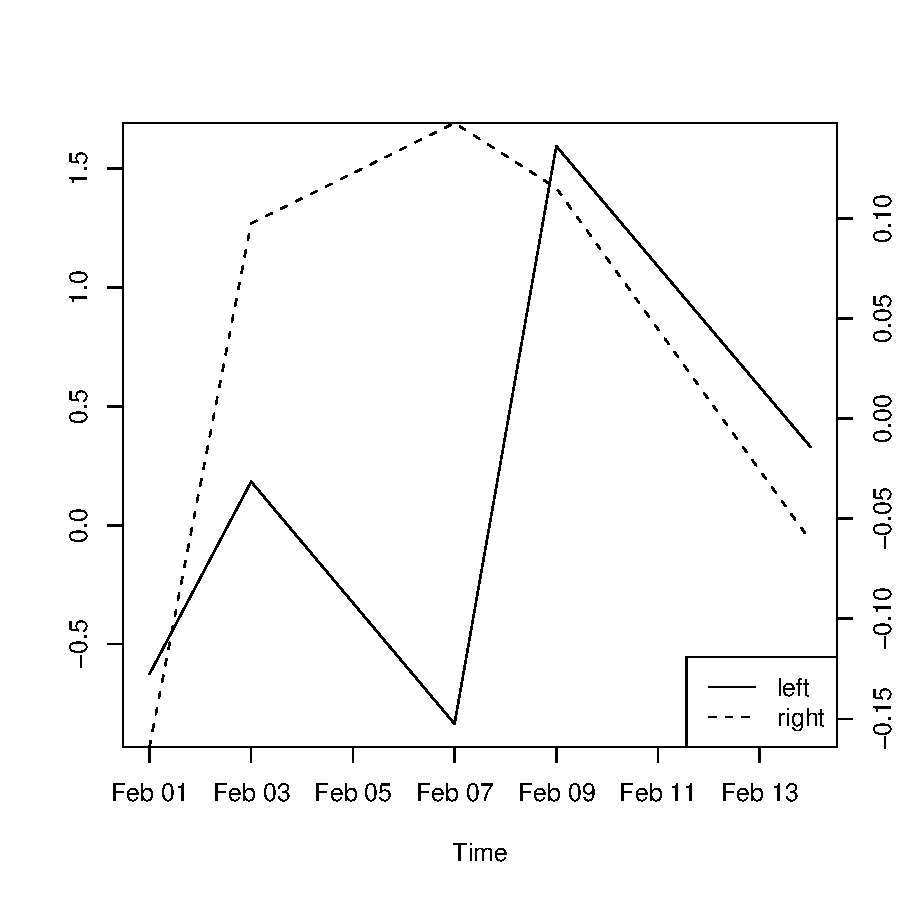
\includegraphics{plot-axes}
\caption{\label{fig:plot-axes} Left and right \code{plot.zoo} axes.}
\end{center}
\end{figure}


\mysection{4. I have data frame with both numeric and factor columns.  How do I convert that to a zoo object?}

A \code{"zoo"} object may be (1) a numeric vector, (2) a numeric matrix or 
(3) a factor but may not contain both a numeric vector and factor.  
Use two \code{"zoo"} variables instead:

\begin{Schunk}
\begin{Sinput}
> DF <- data.frame(time = 1:4, x = 1:4, f = factor(1:4))
> zx <- zoo(DF$x, DF$time)
> zf <- zoo(DF$f, DF$time)
\end{Sinput}
\end{Schunk}

or convert the factor to numeric and create a single
\code{"zoo"} series:

\begin{Schunk}
\begin{Sinput}
> z <- zoo(data.matrix(DF[-1]), DF$time)
\end{Sinput}
\end{Schunk}

\mysection{5. Why does lag these give slightly different results on a zoo and a zooreg series which are otherwise the same?}

To be definite let us consider the following examples, noting how 
both \code{code} and \code{diff} give a different answer with the same 
input except its class is \code{"zoo"} in one case and \code{"zooreg"} in 
another:
\begin{Schunk}
\begin{Sinput}
> z <- zoo(11:15, as.Date("2008-01-01") + c(-4, 1, 2, 3, 6))
> zr <- as.zooreg(z)
> lag(z)
\end{Sinput}
\begin{Soutput}
2007-12-28 2008-01-02 2008-01-03 2008-01-04 
        12         13         14         15 
\end{Soutput}
\begin{Sinput}
> lag(zr)
\end{Sinput}
\begin{Soutput}
2007-12-27 2008-01-01 2008-01-02 2008-01-03 2008-01-06 
        11         12         13         14         15 
\end{Soutput}
\begin{Sinput}
> diff(log(z))
\end{Sinput}
\begin{Soutput}
2008-01-02 2008-01-03 2008-01-04 2008-01-07 
0.08701138 0.08004271 0.07410797 0.06899287 
\end{Soutput}
\begin{Sinput}
> diff(log(zr))
\end{Sinput}
\begin{Soutput}
2008-01-03 2008-01-04 
0.08004271 0.07410797 
\end{Soutput}
\end{Schunk}

\code{lag.zoo} and \code{lag.zooreg} work differently.  For \code{"zoo"}
objects the lagged version is obtained by moving values 
to the adjacent time point that exists in the series but for \code{"zooreg"} 
objects the time is lagged by \code{deltat}, the time between adjacent
regular times.

A key implication is that \code{"zooreg"} can lag a point to a time point
that did not previously exist in the series and, in particular, can lag
a series outside of the original time range whereas that is not possible
in a \code{"zoo"} series.

Note that \code{lag.zoo} has an \code{na.pad=} argument which in some
cases may be what is being sought here.

The difference between \code{diff.zoo} and \code{diff.zooreg} stems from
the fact that \code{diff(x)} is defined in terms of \code{lag} like
this: \code{x-lag(x,-1)}.

\mysection{6. How do I subtract the mean of each month from a zoo series?}

Suppose we have a daily series.
To subtract the mean of Jan 2007 from each day in that month,
subtract the mean of Feb 2007 from each day in that month, etc.
try this:
     
\begin{Schunk}
\begin{Sinput}
> set.seed(123)
> z <- zoo(rnorm(100), as.Date("2007-01-01") + seq(0, by = 10, 
+     length = 100))
> z.demean1 <- z - ave(z, as.yearmon(time(z)))
\end{Sinput}
\end{Schunk}

To subtract the mean of all Januaries from each January, etc.
try this:

\begin{Schunk}
\begin{Sinput}
> z.demean2 <- z - ave(z, format(time(z), "%m"))
\end{Sinput}
\end{Schunk}

\mysection{7. How do I create a monthly series but still keep track of the dates?}

Create a \pkg{S3} subclass of \code{"yearmon"} called \code{"yearmon2"} that 
stores the dates as names on the time vector.  It will be sufficient to create
an \code{as.yearmon2} generic together with an
\code{as.yearmon2.Date} methods as well as the inverse:
\code{as.Date.yearmon2}.
This new class will act the same as \code{"yearmon"} 
stores and allows recovery of the dates using \code{as.Date} and
\code{aggregate.zoo} as shown in the test at the end of this example:

\begin{Schunk}
\begin{Sinput}
> as.yearmon2 <- function(x, ...) UseMethod("as.yearmon2")
> as.yearmon2.Date <- function(x, ...) {
+     y <- as.yearmon(with(as.POSIXlt(x, tz = "GMT"), 1900 + year + 
+         mon/12))
+     names(y) <- x
+     structure(y, class = c("yearmon2", class(y)))
+ }
> as.Date.yearmon2 <- function(x, frac = 0, ...) {
+     if (!is.null(names(x))) 
+         return(as.Date(names(x)))
+     x <- unclass(x)
+     year <- floor(x + 0.001)
+     month <- floor(12 * (x - year) + 1 + 0.5 + 0.001)
+     dd.start <- as.Date(paste(year, month, 1, sep = "-"))
+     dd.end <- dd.start + 32 - as.numeric(format(dd.start + 32, 
+         "%d"))
+     as.Date((1 - frac) * as.numeric(dd.start) + frac * as.numeric(dd.end), 
+         origin = "1970-01-01")
+ }
> dd <- seq(as.Date("2000-01-01"), length = 5, by = 32)
> z <- zoo(1:5, as.yearmon2(dd))
> z
\end{Sinput}
\begin{Soutput}
Jan 2000 Feb 2000 Mar 2000 Apr 2000 May 2000 
       1        2        3        4        5 
\end{Soutput}
\begin{Sinput}
> aggregate(z, as.Date, force)
\end{Sinput}
\begin{Soutput}
2000-01-01 2000-02-02 2000-03-05 2000-04-06 2000-05-08 
         1          2          3          4          5 
\end{Soutput}
\end{Schunk}

\mysection{8. How are axes added to a plot created using plot.zoo?}

On single panel plots \code{axis} or \code{Axis} can be used just as with any 
classic graphics plot in R.

\begin{Schunk}
\begin{Sinput}
> z <- zoo(0:500, as.Date(0:500))
> plot(z, xaxt = "n")
> tt <- time(z)
> m <- unique(as.Date(as.yearmon(tt)))
> jan <- format(m, "%m") == "01"
> mlab <- substr(months(m[!jan]), 1, 1)
> Axis(side = 1, at = m[!jan], labels = mlab, tcl = -0.3, cex.axis = 0.7)
> Axis(side = 1, at = m[jan], labels = format(m[jan], "%y"), tcl = -0.7)
> Axis(side = 1, at = unique(as.Date(as.yearqtr(tt))), labels = FALSE)
\end{Sinput}
\end{Schunk}

A multivariate series can either be plotted as multiple single panel
plots:

\begin{Schunk}
\begin{Sinput}
> z3 <- cbind(z1 = z, z2 = 2 * z, z3 = 3 * z)
> opar <- par(mfrow = c(2, 2))
> tt <- time(z)
> m <- unique(as.Date(as.yearmon(tt)))
> jan <- format(m, "%m") == "01"
> mlab <- substr(months(m[!jan]), 1, 1)
> for (i in 1:ncol(z3)) {
+     plot(z3[, i], xaxt = "n", ylab = colnames(z3)[i], ylim = range(z3))
+     Axis(side = 1, at = m[!jan], labels = mlab, tcl = -0.3, cex.axis = 0.7)
+     Axis(side = 1, at = m[jan], labels = format(m[jan], "%y"), 
+         tcl = -0.7)
+     Axis(side = 1, at = unique(as.Date(as.yearqtr(tt))), labels = FALSE)
+ }
> par(opar)
\end{Sinput}
\end{Schunk}

or as a multipanel plot.  In this case any custom axis must be
placed in a panel function.

\begin{Schunk}
\begin{Sinput}
> plot(z3, screen = 1:3, xaxt = "n", nc = 2, ylim = range(z3), 
+     panel = function(...) {
+         lines(...)
+         panel.number <- parent.frame()$panel.number
+         nser <- parent.frame()$nser
+         if (panel.number%%2 == 0 || panel.number == nser) {
+             tt <- list(...)[[1]]
+             m <- unique(as.Date(as.yearmon(tt)))
+             jan <- format(m, "%m") == "01"
+             mlab <- substr(months(m[!jan]), 1, 1)
+             Axis(side = 1, at = m[!jan], labels = mlab, tcl = -0.3, 
+                 cex.axis = 0.7)
+             Axis(side = 1, at = m[jan], labels = format(m[jan], 
+                 "%y"), tcl = -0.7)
+             Axis(side = 1, at = unique(as.Date(as.yearqtr(tt))), 
+                 labels = FALSE)
+         }
+     })
\end{Sinput}
\end{Schunk}

\mysection{9.  Why is nothing plotted except axes when I plot an 
object with many NAs?}

Isolated points surrounded by \code{NA} values do not form lines 
so try one of the following:

\begin{Schunk}
\begin{Sinput}
> z <- zoo(c(1, NA, 2, NA, 3))
> plot(z)
> plot(z, type = "p")
> plot(na.omit(z))
> plot(na.approx(z))
> plot(z, type = "p")
> lines(na.omit(z))
\end{Sinput}
\end{Schunk}

Note that this is not specific to \pkg{zoo.}  If we
plot in R without zoo we get the same behavior.

\mysection{10. What other packages use zoo?}

\begin{tabular}{|l|p{10cm}|} \hline
\multicolumn{2}{|l|}{\emph{Depends}} \\ \hline
\pkg{BootPR} & Bootstrap prediction intervals and bias-corrected forecasting \\
\pkg{dyn} & Time-series regression \\
\pkg{dynlm} & Dynamic linear regression \\
\pkg{fda} & Functional data analysis \\
\pkg{FinTS} & Companion to Tsay's ``Analysis of financial time series'' \\
\pkg{fUtilities} & \pkg{Rmetrics} function utilities \\
\pkg{fxregime} & Exchange rate regime analysis \\
\pkg{lmtest} & Testing linear regression models \\
\pkg{party} & Recursive partytioning toolbox \\
\pkg{PerformanceAnalytics} & Econometric tools for performance and risk analysis \\
\pkg{quantmod} & Quantitative financial modelling framework \\
\pkg{RBloomberg} & \proglang{R}/\pkg{Bloomberg} interface \\
\pkg{sandwich} & Robust covariance matrix estimators \\
\pkg{strucchange} & Testing, monitoring, and dating structural changes \\
\pkg{tripEstimation} & Metropolis sampler and supporting functions for
  estimating animal movement from archival tags and satellite fixes \\
\pkg{tseries} & Time series analysis and computational finance \\
\pkg{xts} & Extensible time series \\ \hline
\multicolumn{2}{|l|}{\emph{Suggests}} \\ \hline
\pkg{gsubfn} & Utilities for strings and function arguments \\
\pkg{pscl} & Political Science Computational Laboratory, Stanford University \\
\pkg{TSSQLite} & Time series database interface extentions for \pkg{SQLite} \\
\pkg{TSdbi} & Time series database interface \\
\pkg{Zelig} & Everyone's statistical software \\ \hline
\end{tabular}

\end{document}

